% assignment_1.text - Assignment 1 for Machine Learning class (Spring 2015)
% Chanmann Lim - February 2015

\documentclass[a4paper]{article}

\usepackage[margin=1 in]{geometry}
\usepackage{amsmath}
\usepackage{listings}
\usepackage{graphicx}
\usepackage[T1]{fontenc}
\usepackage{float}

\everymath{\displaystyle}

\begin{document}

% Plot 1
\paragraph{1. a} Plot of $p(x|\theta)$\\
\begin{equation}
p(x|\theta = 1) = e^{-x} \quad x \geq 0
\end{equation}
\begin{figure}[H]
  \centering
    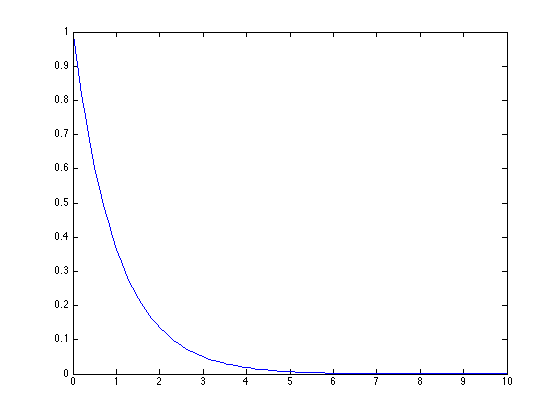
\includegraphics[scale=.52]{images/1_a_1.png}
  \caption{$p(x|\theta) = e^{-x}$}
\end{figure}

% Plot 2
\begin{equation}
p(x = 2|\theta) = \theta e^{-2\theta}
\end{equation}
\begin{figure}[H]
  \centering
    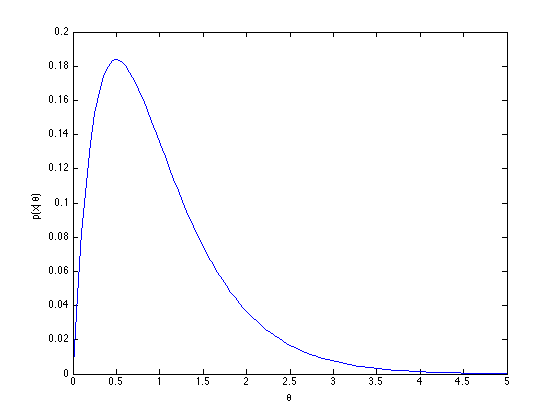
\includegraphics[scale=.52]{images/1_a_2.png}
  \caption{$p(x|\theta) = \theta e^{-2\theta} \quad; 0 \leq \theta \leq 5$}
\end{figure}

\end{document}